\chapter{Método de trabajo}
\label{chap:metodo}
\drop{T}ras haber analizado cuales son los objetivos a desarrollar en el TFG, y realizado un análisis de las tecnologías existentes, es necesario asignar una metodología para la gestión del proyecto. 

Para ello, y valorando el número de personas que están involucradas en el proyecto (director del TFG y su autor), se realiza una investigación sobre cuales son las alternativas de metodologías para llevarlo a cabo, que sea ágil, ligera, y por supuesto, flexible a cambios para adaptar nuevos requisitos que puedan surgir.

Las metodologías Agile, surgen en el año 1990, como herramienta de gestión software que indicase unas correctas directivas para llevar a acabo los proyectos. 

Las metodologías existentes hasta la época, tenían una rigurosa asignación de roles, actividades y artefactos (incluyendo el modelado y una documentación muy detallada), que no obstante, a día de hoy sigue siendo necesaria para proyectos de gran envergadura, que necesitan una alta gestión de tiempo y recursos. 

Según avanza el desarrollo de aplicaciones software, entran en escena nuevas situaciones en las cueles este tipo de métodos de gestión no encaja totalmente con estas metodologías tradicionales. 

Los métodos Agile promueven una gestión de proyectos, que se basa principalmente en fomentar la constante inspección del trabajo y la adaptación de éste. Se trata de un sistema organizado que facilita el trabajo el equipo, una correcta organización, y favorece el rendimiento del tiempo empleado en el desarrollo.

Scrum fue creado, con las características de estos métodos de gestión, trabajando con una comunicación directa y empleando ingeniería concurrente, basándose en las ideas del «Manifiesto por el Desarrollo Ágil de Software» (detalladas en la siguiente sección del documento).

Por lo tanto, basándose en estas ideas, y teniendo en cuenta el número de personas que están involucradas en el proyecto, se ha elegido la metodología de trabajo Scrum.


\section{Metodología Agile}



\section{Scrum como metodología de trabajo}



\subsection{Roles}



\subsection{Artefactos}



\subsection{Motivos de la elección del método Scrum}



\section{Aplicación del método de trabajo}



\subsection{Iteración 1 : Inicio del TFG }
En esta primera iteración el objetivo es conocer el alcance del proyecto, entendiendo que hay que construir, realizando un estudio los actuales sistemas tangibles enfocados a la programación tangible para niños, y que tecnología y características utilizan cada uno de ellos, para poder identificar cuales son los puntos que se pueden mejorar en esos sistemas y contribuir a mejoralos, diseñando una plataforma de juego que resuelva todos esos puntos. Este analisis premitira establecer que requisitos debe tener la plataforma a diseñar, y que tecnologias utilizar en ella, para posteriormente establecer los pasos a realizar para alcanzar una serie de objetivos especificos dentro de la aplicación.

En el «Capítulo Antecedentes» de este documento, se muestran los resultados sobre los principales estudios experimentales aplicados a la interacción tangible y como motiva a niños de tempranas edades en sus habilidades computacionales. Se muestran algunos de los dispositivos mas importantes y que aportan diferentes enfoques en la interacción tangible y que han sido utilizados para el aprendizaje computacional, así como sus características y tecnología utilizada.

Finalmente se exponen las areas en los actuales sistemas tangibles.

\subsection{Áreas de mejora en sistemas tangibles.}
Los diferentes sistemas de interacción tangible tienen como propósito general, que la
información sea comprensible y literalmente captable, haciendo uso de objetos físicos
que sean manipulables de una forma natural.\\
Otra de las características de la aplicación de los sistemas tangibles en el ámbito
educativo, es que el entorno visual debe motivar fuertemente al usuario, disponiendo
de un entorno de fácil uso e intuitivo, y que, además, fomente la capacidad de
razonamiento, creación e imaginación de los niños.\\
La evolución de la tecnología aplicada a los modelos actuales de sistemas tangibles, van
adaptándose para mejorar los diseños y conseguir de esta forma sistemas más fiables.
No obstante, existen diferentes áreas de mejora localizadas sobre los diferentes
sistemas de interacción tangible:
\begin{itemize}
\item Uso de elementos externos para su funcionamiento: en algunos juegos, es
imprescindible es uso de un ordenador para su normal funcionamiento (como es
el caso de Scratch \& WeDo), además del uso de periféricos, por ejemplo, el uso
de una cámara para el reconocimiento de imágenes.
\item Elevado número de elementos tangibles para el desarrollo del juego: si bien es
cierto, que uno de los puntos más importantes a la hora de la programación para
niños, es poder representar partes de código de diferentes elementos tangibles,
un gran número de elementos puede suponer un problema para el niño a la hora
del desarrollo del juego, pudiendo en algunos casos confundirlo.
\item Enfoque exclusivo de un rango de edades para el juego: en la mayoría de los
casos, los juegos están enfocados a niños de un determinado rango de edades,
limitando de esta manera el juego, ya que puede resultar de una dificultad
elevada para niños de corta edad, o demasiado fáciles para el resto de edades.
\item Diseño estático del juego: una de las limitaciones de todos los juegos que hacen
uso de interfaces tangibles, es que no pueden ser actualizados, o no disponen de
actualizaciones de software, lo que hace que el juego no evolucione, e
imposibilita posibles futuras mejoras en los juegos.
\item Alto coste de los bloques o dispositivos de realimentación: el uso de un gran
número de elementos utilizados para la interacción tangible, eleva el precio del
diseño.
\end{itemize}


\subsection{Iteración 2: Establecer Requisitos Iniciales e Investigación sobre las Tecnologías a Utilizar}

Las áreas de mejora obtenidas en la Iteración 1 serviran de base para realizar la plataforma de juego. Se analiza cada punto para obtener la mejor solución posible y que tecnología utilizar para cada caso.

\subsubsection{Uso de elementos externos al dispositivo}
El uso de elementos externos para el funcionamiento del juego, como por ejemplo el uso de un teclado o una pantalla que el propio usuario ya debe de disponer, en ocasiones puede acarrear un problema a la hora de utilizar el juego.\\ 
Para eliminar el uso de elementos externos para el funcionamiento del sistema de juego, se ha de conseguir diseñar un prototipo el cual prescida de dichos elementos, integrando todo lo necesario dentro de la misma plataforma. Por lo tanto el primer requisito a implementar es: \textbf{Dispositivo completo e independiente de elementos externos al mismo.}

\subsubsection{Elevado número de piezas para la interacción tangible}
Un sistema de interacción tangible se caracteriza principalmente en que la información sea comprensible y literalmente captable, haciendo uso de objetos físicos que sean manipulables de forma natural. En ocasiones, el número de objetos físicos para el desarrollo del juego es elevado. Si bien es cierto que uno de los puntos más importantes a la hora de la programación para niños, es poder representar partes de código en diferentes elementos tangibles, un gran número de elementos puede suponer un problema para el niño a la hora del desarrollo del juego, pudiendo en algunos casos confundirlo. 

Los sistemas de programación tangible utilizan bloques que al conectarlos o posicionarlos de una manera concreta, generan en tiempo real movimientos o acciones, bien mostrando la acción realizada en una pantalla, o bien mediante algún tipo de robot articulado, etc... Cada bloque indica una acción, por ejemplo bloque de inicio, bloque de fin, bloque de dirección, bloque sensor... 

Para dar solución a este problema, la idea pasa por intentar agrupar los bloques tangibles que son utilizados en los actuales juegos y que tienen como finalidad representar una acción, en un solo elemento tangible.

Se propone el diseño de un dispositivo tangible, que por medio de un microprocesador, muestre en una pantalla estas funciones. 
Por tanto, el segundo de los requisitos es: \textbf{Agrupar los elementos tangibles que realizan las funciones en un solo dispositivo tangible.}


\subsubsection{Enfoque exclusivo del juego en un rango de edades y diseño estático del juego}

Uno de los puntos mas importantes de a tratar es el que la mayoria de los diseños actuales esta enfocado a un rango de edades para el juego, ya que un determinado tipo de juego puede resultar demasiado simple o demasiado complejo para algunos niños, debido a la edad de los mismos. 

Otro punto a tener en consideración es el diseño estático en los juegos de interacción tangible. El usuario dispone de unos recursos para ser utilizados, y aunque las combinaciones y posiciones de elementos tangibles permitan realizar diferentes acciones de juego, no dejan de ser siempre los mismos elementos con los mismos propositos.

Estos dos puntos estan relacionados con una caracteristica común, y es que no tienen la posibilidad de mejorar, no pueden ser actualizdos, al menos que se compre una nueva versión del producto, lo perjudica al usuario final.

Por tanto, el siguiente requisito para el diseño es: \textbf{Disponer de actualizaciones software para posibles mejoras en los juegos.}

\textbf{Alto coste de los bloques o dispositivos de realimentación}
El alto coste de los bloques o dispositivos de realimentación al igual que el uso de un gran número de elementos utilizados para la interacción tangible, eleva el precio del
diseño.
El ultimo de los requisitos es: \textbf{Utilización de elementos de bajo coste para el diseño}





Este elemento ha sido denominado con el nombre de «TUIO2» (Tangible User Interface Object).

El dispositivo TUIO2 por si solo no tiene sentido, ya que necesita de algun medio de representación de todas estas funciones. Para ello se ha diseñado el dispositivo tangible «TUIO1», que dispone al igual que el elemento TUIO2, de un microprocesador y una pantalla que permite la representación de estas funciones al interactuar TUIO2 con TUIO1. Este medio de interacción se realiza posicionando TUIO2 sobre la pantalla de TUIO1.

Ambos dispositivos son comunicados entre sí para intercambio de información, mediante comunicación wifi.

TUIO2 en su parte inferior tiene tres almohadillas conductivas posicionadas de tal forma que generan un patrón de coordenadas, que al posicionarse sobre la pantalla de TUIO1, que es capacitiva, detecta la posición y ángulo de TUIO2, estableciendose comunicación entre ambos dispositivos para mandar la información necesaria. La pantalla de TUIO1 muestra las funciones que han sido añadidas, para finalmente realizar la acción que se pretende, siendo dicha acción visualizada en la pantallade TUIO1.

Este tipo de interacción entre ambos elementos no solo se utiliza para añadir funciones desde TUIO2 y que TUIO1 las represente y realice la acción, sino que tambien ofrece la posibilidad de que la acción sea «capturada» por el elemento TUIO2 y que el juego se desarrolle en ambas pantallas, ampliando de esa manera las posibilidades de interacción

El elemento TUOI2 incorpora un sensor inercial, el cual sirve para manejar.........






\subsection{Iteración : Sistema de localización del Widget tangible sobre la pantalla táctil}
Uno de los objetivos principales de este TFG es diseñar y programar un sistema de localización y reconocimiento entre las dos interfaces de usuario tangibles. Este sistema de localización consiste en obtener las coordenadas de la posición del «Widget tangible» sobre la pantalla táctil capacitiva del dispositivo TUIO1. Estas coordenadas son enviadas desde TUIO1 a TUIO2. Lo que se quiere obtener es una representación en la pantalla de TUIO2 de la imagen o animación de lo que muestra la pantalla de TUIO1.\\
Antes de posicionar TUIO2 sobre TUIO1, las pantallas de ambos dispositivos muestran imágenes diferentes (ver Figura~\ref{fig:Localizacion1}).
\begin{figure}[!h]
\begin{center}
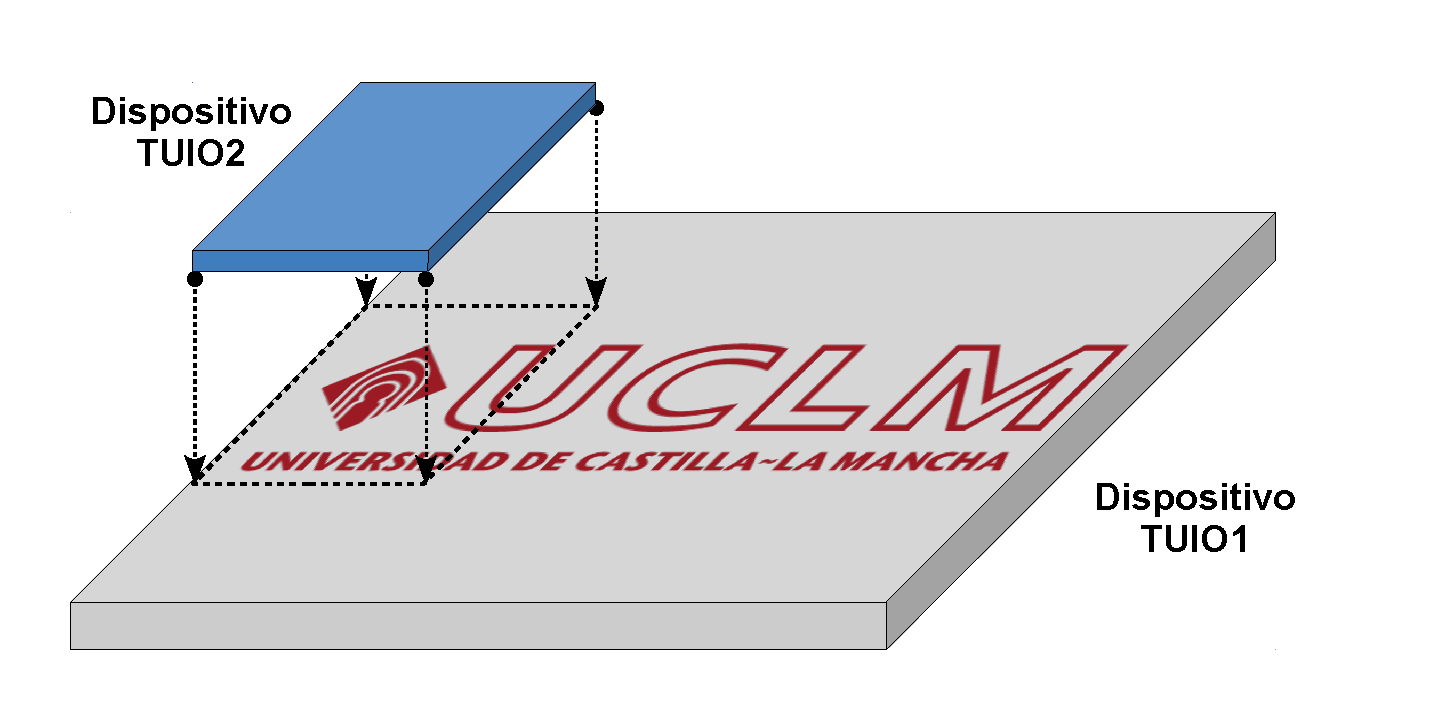
\includegraphics[width=0.7\textwidth]{localizacion1.pdf}
\caption{Posición de los dispositivos antes de la interacción sobre la pantalla capacitiva}
\label{fig:Localizacion1}
\end{center}
\end{figure}
Al posicionar TUIO2 sobre la pantalla de TUIO1, la pantalla de TUIO2 muestra la parte de imagen correspondiente que es tapada por el dispositivo como se muestra en la Figura~\ref{fig:Localizacion2}:
\begin{figure}[!h]
\begin{center}
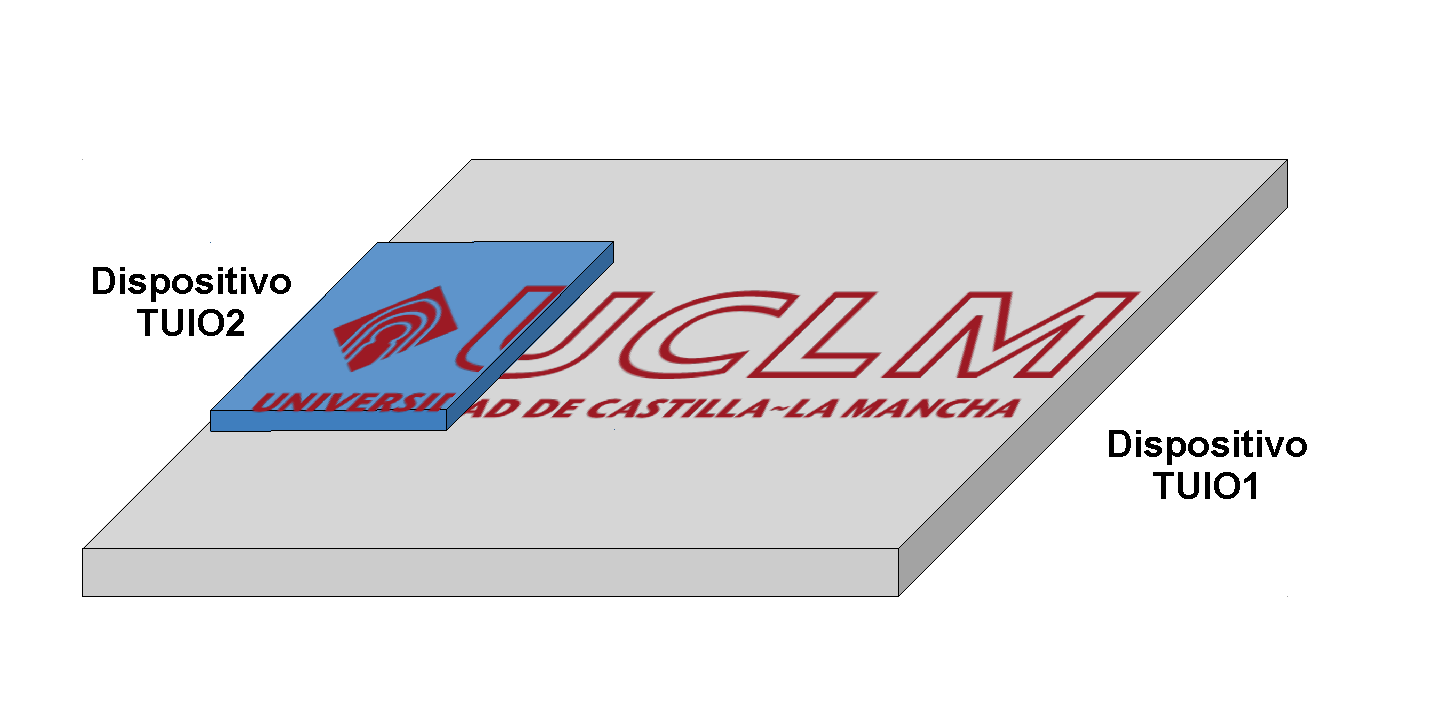
\includegraphics[width=0.7\textwidth]{localizacion2.pdf}
\caption{Posición de los dispositivos despues de la interacción sobre la pantalla capacitiva}
\label{fig:Localizacion2}
\end{center}
\end{figure}


\subsubsection{Localización del Widget tangible TUIO2}

El procedimiento para obtener la posición de del dispositivo TUIO2 sobre la pantalla del dispositivo TUIO1, se consigue mediante el uso del sensor capacitivo de la propia pantalla de TUIO1, que al detectar una variación de la capacitancia genera un evento táctil.
El dispositivo TUIO2 produce tres eventos táctiles sobre la pantalla capacitiva. Estos eventos son generados por medio de tres almohadillas de goma conductora que están conectadas al borne negativo de la «RaspberryPi». Esta conexión evita que el usuario tenga que sostener con su propia mano el dispositivo, haciendo de conexión a tierra el propio borne negativo.
El diseño de los puntos de contacto es el que se muestra en la siguiente Figura~\ref{fig:Localizacion3}.
\begin{figure}[!h]
\begin{center}
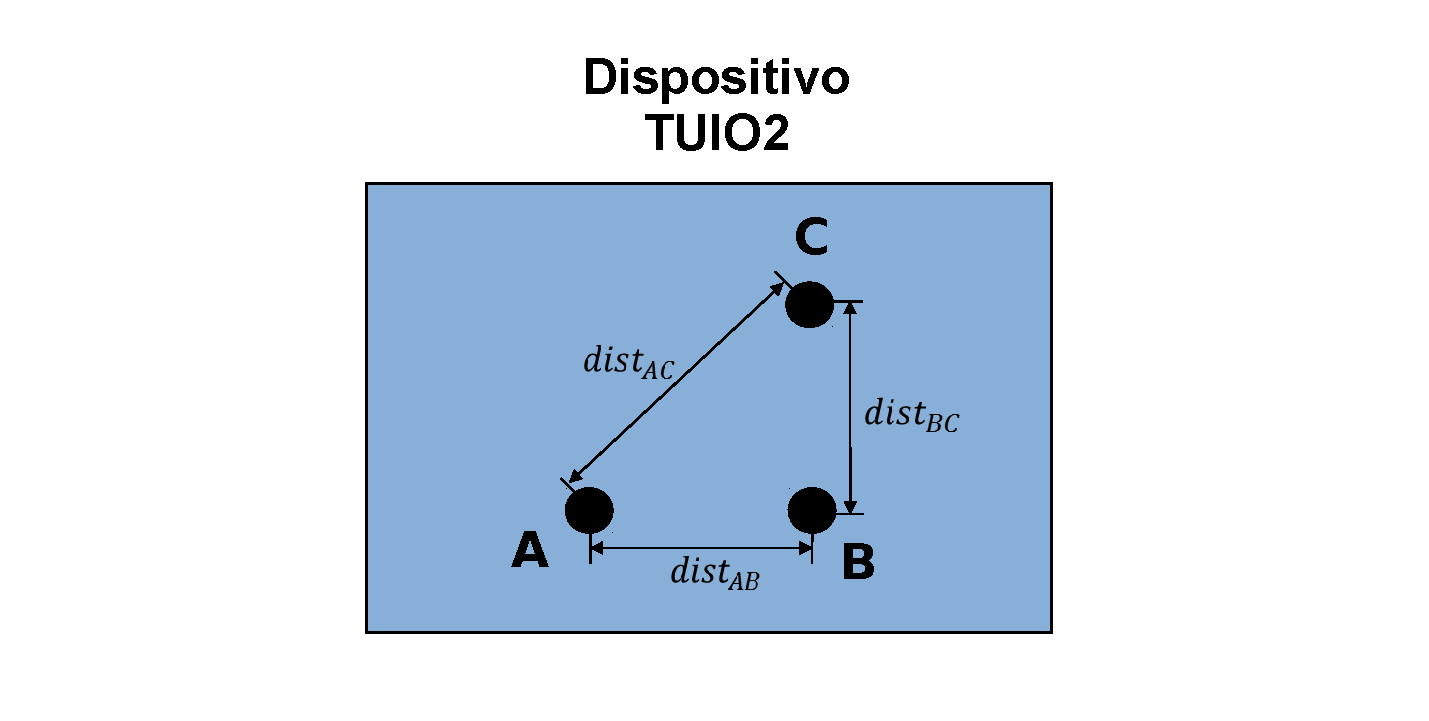
\includegraphics[width=0.9\textwidth]{localizacion3.pdf}
\caption{Disposición de las almohadillas conductoras en la parte inferior del «Widget tangible» para generar los eventos táctiles. }
\label{fig:Localizacion3}
\end{center}
\end{figure}
Los tres puntos de contacto son identificados A, B y C, que dan nombre a los vértices del triángulo rectángulo escaleno que forman. Se ha elegido este tipo de diseño ya que cada uno de los tres lados tiene una medida diferente, lo que hace que sea mas fácil identificar cada segmento del triangulo y así evitar posibles problemas cuando se localice cualquiera de sus vértices.

Cuando TUIO2 está sobre la pantalla, los eventos táctiles generados proporcionan la siguiente información al dispositivo TUIO1: posición e ID del evento. Las coordenadas de la posición de cada evento táctil es medida en pixels, por lo que cada evento producido será manejado en esas unidades de media (ver Figura~\ref{fig:Localizacion4}).\\
\begin{figure}[!h]
\begin{center}
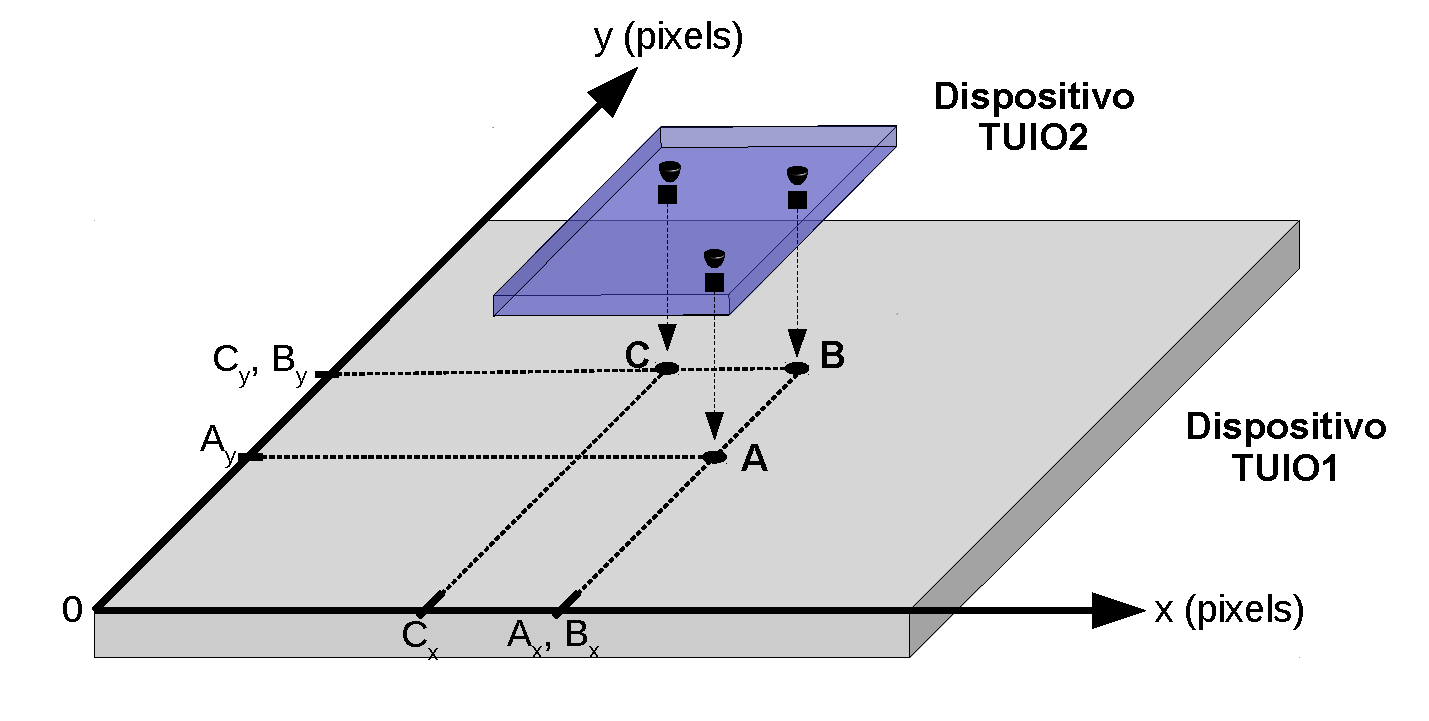
\includegraphics[width=0.9\textwidth]{localizacion4.pdf}
\caption{Coordenadas de los puntos A, B y C del «Widget tangible» sobre la pantalla capacitiva. }
\label{fig:Localizacion4}
\end{center}
\end{figure}
Estos datos son interpretados y tratados para calcular la posición de TUIO2 mediante un programa en «Python».

\subsubsection{Programa para la localización.}

Todos los eventos táctiles generados sobre la pantalla capacitiva del dispositivo TUIO1 son manejados por la \textit{clase Widget} en «Kivy», mediante el método \texttt{on\_touch\_down().}\\
Este método obtiene la información de posición e ID del evento táctil producido, almacenando estos datos en la lista \texttt{touch[].}\\
Se crea una librería específica para el manejo de esta lista, la cual se tratará y manejara los datos para obtener la información de posición de TUIO2.

\textbf{Método \texttt{pulsacion(touch)}}\\
El argumento de entrada corresponde con las coordenadas y la id del evento táctil que contiene la lista de eventos (\texttt{touch}).\\
Estos datos son almacenados en la última posición de la lista \texttt{puls[]} mediante el método \texttt{append()}:\\
\texttt{self.puls.append((t.x,t.y,t.id))}.\\
donde: \\
\texttt{t.x}: coordenada x del evento táctil.\\
\texttt{t.y}: coordenada y del evento táctil.\\
\texttt{t.id}: identificación del evento táctil (número de evento).\\
Cuando el número de eventos almacenados en \texttt{puls[]}   
es mayor que 1, se llama al método \texttt{determinar\_distancias()}.

\textbf{Método \texttt{determinar\_distancias()}}.\\
Mediante el método \texttt{Vector()}, de la librería \texttt{kivy}, es determinada la distancia entre los eventos táctiles producidos hasta el momento, y que son almacenados en la lista \texttt{puls[]}, haciendo uso de un bucle el cual recorre desde el último elemento de la lista \texttt{puls[]} hasta el primero. El método \texttt{determinar\_lados} es llamado en cada medida que se realiza de la distancia. Si la distancia es correcta, se incrementa la variable \texttt{contador}, la cual al llegar a 2, llama al método \texttt{determinar\_puntos()}.

\textbf{Método \texttt{determinar\_lados()}}.\\
Método para verificar si los dos eventos táctiles de los cuales se han determinado la distancia, corresponden con uno de los lados del triángulo del \textit{Widget tangible}, donde \textit{m} corresponde con la distancia entre los dos eventos táctiles, \textit{i} el tamaño de la lista \texttt{puls[]}, y \textit{a} el número de iteración del bucle que recorre cada uno de los elementos de la lista \texttt{puls[]}.

Este método es llamado cada vez que el método \texttt{determinar\_distancias()} es invocado.
Se comprueba si la distancia entre los dos puntos corresponde con el rango de medidas establecidos para los lados del triangulo del \emph{Widget tangible}. Los rangos de medida son los mostrados en la siguiente tabla (~\ref{tab:intervalos-coordenadas}).

\begin{table}[hp]
  \centering
  {\small
  


\begin{tabular}{p{.2\textwidth}p{.2\textwidth}}
  \tabheadformat
  \tabhead{Rango}   &
  \tabhead{Segmento del triángulo}  \\
\hline
(120,150) & AB \\
\hline
(160,150) & BC \\
\hline
(210,260) & AC
\end{tabular}


% Local variables:
%   coding: utf-8
%   ispell-local-dictionary: "castellano8"
%   TeX-master: "main.tex"
% End:

  }
  \caption[Intervalos de medida de cada segmento del triángulo]
  {Intervalos de medida de cada segmento del triángulo}
  \label{tab:intervalos-coordenadas}
\end{table}
Si la medida corresponde con alguno de los rangos establecidos, dicha medida es almacenada junto con las coordenadas de ambos eventos en la lista \texttt{dist[]}. Por ejemplo si la distancia entre los dos eventos táctiles es correcta y corresponde al segmento AB, los datos en la lista \texttt{dist[]} son almacenados de la siguiente manera:\\
\texttt{self.dist.append((m,'AB',toq1,toq2)) }\\
donde \texttt{m} corresponde a la distancia entre ambos puntos, \texttt{AB} es el nombre del segmento al que corresponde, \texttt{toq1} son las coordenadas del evento táctil con el cual se está midiendo la distancia en el método \texttt{determinar\_distancias()}, y \texttt{toq2} son las coordenadas del ultimo evento táctil.
Si la distancia es correcta se incrementa en una unidad la variable \texttt{contador}.

\textbf{Método \texttt{determinar\_puntos()}}.\\
Este método es invocado dentro del método \texttt{determinar\_distancias()} cuando la variable \texttt{contador} es mayor a 1, es decir, existen dos segmentos correctos del triángulo cuyos datos han sido almacenados en la lista \texttt{dist[]}, la cual contiene en ese momento dos elementos.
Los puntos del triangulo (A,B,C), son determinados siguiendo la siguiente lógica:
Por ejemplo, si los segmentos de los elementos de \texttt{dist[]} corresponden con $\overline{BC}$ y  $\overline{AB}$ respectivamente, se llama al método \texttt{asignar\_puntos}, donde los argumentos de entrada se establecen de la manera que sigue:

\texttt{self.asignar\_puntos(1,2,0,'B','C','A')}\\

A continuación se procede a detallar el método \texttt{asignar\_puntos}.

\textbf{Método \texttt{asignar\_puntos()}}.\\
Mediante este método se asigna a cada vértice A, B y C del triángulo, las coordenadas donde se encuentra cada uno de ellos, al igual que el nombre del vertice, y se almacenan dichos datos en la lista \texttt{coordenadas[]}

Para establecer un orden a la hora de añadir los valores a la lista \texttt{coordenadas[]} se pasa como argumentos la posición a la que corresponden cada uno de los puntos.\\
0: corresponde a la posición de la letra A en la lista \texttt{coordenadas[].}\\
1: posición de la letra B para la lista \texttt{coordenadas[]}.\\
2: posición de la letra C en la lista \texttt{coordenadas[]}.\\

La finalidad es que la lista \texttt{coordenadas} quede con la siguiente estructura para ser 
manejada:\\

$[(x_{A},y_{A},'A'),(x_{B},y_{B},'B'),(x_{C},y_{C},'C')]$\\

En el ejemplo anterior teniamos que los elementos de \texttt{dist[]} corresponden con $\overline{BC}$ y $\overline{AB}$. El punto en común para ambos segmentos corresponde a \textit{\textit{B}}, \textit{C} para el primer segmento, y \textit{A} para el segundo segmento
La llamada al método para asignar los puntos es:\\
\texttt{self.asignar\_puntos(1,2,0,'B','C','A')}\\
donde los argumentos de entrada son:
c = 1, posición del punto en común entre los dos segmentos. Como el punto en comun es \textit{B} que corresponde con la posición 1 de la lista \texttt{coordenadas[]}.\\
c1 = 2, es la posición del punto \textit{C} para el ejemplo, según el criterio establecido.\\
c2 = 0, corresponde a la posición del punto \textit{A} para la lista \texttt{coordenadas[]}.\\
p = 'B', Nombre del vértice en común, en este ejemplo corresponde al vértice \textit{B}.\\
p1 = 'C', Nombre del vértice restante del primer segmento, en este caso el primer segmento es el $\overline{BC}$, por lo tanto el vértice corresponde al \textit{C}.\\
p2 = 'A', Nombre del vértice del segundo segmento, que corresponde con el vértice \textit{A}.\\

Siguiendo con el ejemplo, los valores que contiene la lista \texttt{dist[]} para ser manejados por el método \texttt{asignar\_puntos()} son:
\texttt{[(0, 'NADA'), (164.0, 'BC', (440.00000000000006, 346.0, 'mouse2'), (440.00000000000006, 182.0, 'mouse1')), (134.03357788255903, 'AB', (306.0, 179.0, 'mouse3'), (440.00000000000006, 182.0, 'mouse1'))]}\\

La lista es recorrida mediante el siguiente bucle (ver Listado~\ref{code:buclevertices}):
\begin{lstlisting}[
  float    = ht,  
  language = python,
  caption  = {«Bucle para asignar las coordenadas de los vértices»},
  label    = code:buclevertices]
for a in r
	for b in range(2):
		if self.dist[1][a+2][2] == self.dist[2][b+2][2]:
			self.coordenadas[c] = (self.dist[1][a+2][0],self.dist[1][a+2][1],p)
			if a == 0:
				self.coordenadas[c1] = (self.dist[1][3][0],self.dist[1][3][1],p1)
			else:
				self.coordenadas[c1] = (self.dist[1][2][0],self.dist[1][2][1],p1)
			if b == 0:
				self.coordenadas[c2] = (self.dist[2][3][0],self.dist[2][3][1],p2)
			else:
				self.coordenadas[c2] = (self.dist[2][2][0],self.dist[2][2][1],p2)
			break
\end{lstlisting}
Donde \texttt{a} es la posición para el primer elemento de la lista \texttt{dist[]}, y \texttt{b} la posición del segundo elemento de la lista \texttt{dist[]}

El bucle busca cuales son las coordenadas en común entre los dos segmentos del triangulo. La lista \texttt{dist[]} contiene dos elementos que son los dos segmentos del triangulo con las coordenadas de los eventos táctiles, por lo tanto se recorre las coordenadas de los segmentos buscando la \textit{id} en común. 

Para poder analizar mejor este ejemplo, separamos los dos elementos de la lista \texttt{dist[]}:\\

\texttt{Elemento 1 de dist[]}:\\
\texttt{(164.0, 'BC', (440.00000000000006, 346.0, 'mouse2'), (440.00000000000006, 182.0, 'mouse1'))}\\

\texttt{Elemento 2 de dist[]}:\\
\texttt{(134.03357788255903, 'AB', (306.0, 179.0, 'mouse3'), (440.00000000000006, 182.0, 'mouse1'))}\\

La \textit{posición 0} corresponde a la distancia entre segmentos, la \textit{posición 1} es el nombre del segmento, y las dos restantes posiciones son las coordenadas de los puntos del segmento junto con la \textit{id} del evento táctil.\\

\texttt{id: 'mouse1'} es el elemento en común para los dos segmentos, en este caso $\overline{BC}$ y $\overline{AB}$, donde el punto en común es el punto \textit{B}. Por lo tanto para el ejemplo:\\

\texttt{self.coordenadas[c] = (self.dist[1][a+2][0],self.dist[1][a+2][1],p)}\\

Las coordenadas del punto \textit{B} (coordenada x y coordenada y) son almacenadas en la lista \texttt{coordenadas[]}, al igual que el nombre del vértice común (argumento \texttt{p = 'B'}), en la posicion \texttt{c}, que como argumento de entrada se indicó como 1 (punto \textit{B}). 

La posición de \textit{'mouse1'} para el primer elemento de \texttt{dist[]}, es para un valor de \texttt{a} igual a 1 (ya que al valor de \texttt{a} se le suma 2 posiciones, por ser los dos primeras la distancia entre segmentos, y el nombre del segmento), es decir, la posición 3 del elemento 1 de \texttt{dist[]}.\\

Para el segundo elemento, la posición del vértice \textit{B} corresponde a un valor de \texttt{b = 1} como en el caso del primer segmento.
Una vez asignada las coordenadas del punto en común, el nombre del vértice, y almacenados dichos datos en la lista \texttt{coordenadas[]} en la posición 1, son determinadas las coordenadas de los dos puntos restantes del triángulo (\textbf{C} y \textit{A}): 
Con los tres vértices del triángulo, se calcula el área del triangulo mediante la llamada al método \texttt{calculo\_area}, para verificar que el triangulo es correcto y corresponde con las posiciones del «Widget tangible» y no responde a un error de eventos sobre la pantalla táctil.\\

\textbf{Método \texttt{calculo\_area()}}.\\
El método \texttt{calculo\_area}, retorna el valor del área, la cual, se debe encontrar en el intervalo (9545,16000). 
Si el área no es correcta, se realiza una llamada al método \texttt{inicializar\_a\_0}, para restablecer los valores a sus condiciones iniciales. 
Si el área esta dentro del intervalo establecido, se invoca el método \texttt{mandar\_datos}, el cual enviá los datos de coordenadas de los vértices y el ángulo que forma el «Widget tangible» sobre la pantalla táctil.\\ 
El cálculo del ángulo es realizado por el método \texttt{calculo\_angulo}.
Este método realiza un cálculo del área del triángulo formado sobre la pantalla mediante la regla de Sarrus (determinante).
El argumento de estrada es la lista \texttt{coordenadas[]} que contiene las coordenadas de los vértices del triángulo:\\
\texttt{det = abs((c[0][0]*c[1][1])+(c[0][1]*c[2][0])+(c[2][1]*c[1][0])}\\
\texttt{-((c[1][1]*c[2][0])+(c[0][1]*c[1][0])+(c[0][0]*c[2][1])))*0.5}.\\

\subsection{Iteración : Interfaces gráficas de los dispositivos}

La interfaz gráfica ha sido desarrollada mediante la biblioteca Kivy de Python y consta de una pantalla principal, pantalla de juegos, pantalla de ayuda y pantalla de configuración. Ambos dispositivos han sido diseñados mediante el mismo método de administración de pantallas.\\
Para acceder a cada una de las pantallas, se ha diseñado un menú en la parte superior de la aplicación. Este menú siempre es visible, y permite navegar por las pantallas de una forma directa.\\
Las diferentes pantallas son administradas mediante la biblioteca ScreenManager de Kivy.
ScreenManager es un widget dedicado a administrar múltiples pantallas para aplicaciones y muestra solo una pantalla a la vez en cada una de las transiciones.\\
Cada una de las pantallas corresponde con un archivo en lenguaje KV, y por lo tanto, de extensión .kv. Estos archivos están localizados en la carpeta data/pantallas de la carpeta raíz de la aplicación.\\
Los iconos y fondos de pantalla utilizados en la aplicación para la interfaz se encuentran en la carpeta data/icons y data/fondos respectivamente de la carpeta raíz.\\

\subsubsection{Método de administración de pantallas ScreenManager en Python.}
El método constructor \texttt{build()} de la aplicación principal dispone de las siguientes declaraciones para el administrador de pantallas:
\begin{lstlisting}[
  float    = ht,  
  language = python,
  caption  = {«Inicialización de las pantallas disponibles para el administrador de pantallas ScreenManager para el dispositivo Principal»},
  label    = code:initscreens]
#Objeto dedicado a almacenar los datos de los archivos .kv de cada una
#de las pantallas
self.pantallas = {}
#Listado de las pantallas disponibles
self.pantallas_disponibles = sorted([
            			'PantallaPrincipal','PantallaJuegos','PantallaAyuda',
            			'PantallaConfigurar','PantallaJuego1','PantallaJuego2',
            			'PantallaJuego3' ])
#Copia de los nombres de las pantallas
self.screen_names = self.pantallas_disponibles
#Se crea un listado con la ruta de cada una de las pantallas en formato .kv
directorio = dirname(__file__)
self.pantallas_disponibles = [join(directorio, 'data', 'pantallas',
	'{}.kv'.format(fn).lower()) for fn in self.pantallas_disponibles]

#Cargar toda la lista de pantallas disponibles.
for i in range(len(self.pantallas_disponibles)-1):
	self.go_screen(i)

#Cargar la pantalla principal
idx = self.screen_names.index('PantallaPrincipal')
self.go_screen(idx)
\end{lstlisting}

La función principal es manejar cada una de las pantallas que dispone la aplicación. Se crea un listado con los nombres de las pantallas y otro listado con la ruta donde se encuentran los archivos con el código en lenguaje KV. Posteriormente se carga cada una de las pantallas mediante el método \texttt{go\_screen}.\\

\begin{lstlisting}[
  float    = ht,  
  language = python,
  caption  = {«Método \texttt{go\_screen(), método \texttt{cargar\_pantalla()}} y método \texttt{switch\_to} de ScreenManager»},
  label    = code:cargarpantallas]
#Metodo para cargar el codigo de la pantalla
def cargar_pantalla(self, index):
	if index in self.pantallas:
		return self.pantallas[index]
	screen = Builder.load_file(self.pantallas_disponibles[index])
	self.pantallas[index] = screen
	return screen

	#Metodo para mostrar la pantalla deseada
def go_screen(self, idx):
	self.index = idx
	self.root.ids.sm.switch_to(self.cargar_pantalla(idx), direction='left')
\end{lstlisting}

El método\texttt{go\_screen()} tiene como argumento de entrada el nombre de la pantalla que se quiere mostrar. A su vez se invoca al método \texttt{switch\_to} de \textbf{ScreenManager}, cuya función principal es la de cambiar de pantalla. Los argumentos que utiliza de entrada son el archivo \.kv de la pantalla, y las opciones de desplazamiento. La entrada del archivo con extensión .kv y que contiene el código de la pantalla que se quiere mostrar, se realiza mediante el método \texttt{cargar\_pantalla()}.

\subsubsection{Método de administración de pantallas ScreenManager en Kivy.}
La administración de las pantallas mediante ScreenManager en Kivy es relativamente sencilla en cuestión de código se refiere. En el archivo KV, en la clase principal de la aplicación, la cual es denominada \texttt{Itanium}, tiene la declaración inicial de ScreenManager, la cual se identifica con \texttt{id: sm} como se muestra en el siguiente listado \label{ScreenManager}:
\begin{lstlisting}[
  float    = ht,  
  language = python,
  caption  = {«Forma de inicializar ScreenManager en el archivo KV principal de la aplicación»},
  label    = code:ScreenManager]
<Itanium>:
    ScreenManager:
        id: sm
\end{lstlisting}

Al cargar una pantalla, el archivo que corresponde a cada una de ellas, debe tener en el encabezado el nombre de la clase principal de la aplicación, seguido del nombre de indentificación \texttt{id}, que se especificó en el constructor de la aplicación como se muestra en el siguiente ejemplo \label{sm_ejemplo}:

\begin{lstlisting}[
  float    = ht,  
  language = python,
  caption  = {«Etiqueta en ScreenManager para identificar la pantalla»},
  label    = code:sm_ejemplo]
Itanium:
    name: "PantallaJuegos"
\end{lstlisting}

\subsubsection{Barra de acción para el manejo de pantallas.}
Una vez establecida la forma de mostrar e identificar las pantallas que dispone la aplicación, es necesario navegar por ellas de una forma fácil y rápida. Para ello se ha diseñado una barra de menú que se encuentra en la parte superior de la aplicación, y que muestra un icono para la navegación por pantallas, al igual que un icono que indica la conexión entre ambos dispositivos, y un botón de apagado de la aplicación.

Esta barra de acción es declarada dentro del archivo KV de la aplicación principal, y en ella se indica los distintos elementos que la componen (ver Figura:\label{barra_menu}).  
\begin{figure}[!h]
\begin{center}

\includegraphics[width=0.9\textwidth]{barra_menu.pdf}
\caption{Barra de acción utilizada en el dispositivo principal. }
\label{fig:barra_menu}
\end{center}
\end{figure}


